\scanpage{60}
\figure{\begin{tikzpicture}[x=.008cm,y=-.008cm,line width=.2pt,every node/.style={font=\small,inner sep=1pt}]
\node at (1155,171) {$13/15<\dfrac{7}{8}$};
\node at (1129,323) {$\dfrac{3}{4}>\dfrac{11}{15}$};
\node at (1133,416) {$\dfrac{2}{3}<\dfrac{11}{16}$};
\node at (1129,526) {$\unsure{\dfrac{6}{11}}\unsure{\geq|\neq}\dfrac{1}{2}$};
\node at (485,441) {$\dfrac{12}{14}=\dfrac{6}{7}$};
\draw (47,1140)--(1057,1123);
\draw (47,1127)--(47,1140)--(175,1077)--(1048,305);
\draw (111,1140)--(175,1077)--(236,1014)--(300,949)--(361,885)--(609,692)--(670,629)--(1048,305);
\draw[very thin] (47,1140)--(300,918)--(609,657)--(1048,305);
\draw[very thin] (111,1140)--(361,914)--(670,638)--(1048,305);
\foreach \x/\y in {47/1140,111/1140,175/1077,236/1014,300/949,361/885,609/692,670/629,1048/305,1049/624,1053/811,1054/875}
 {\fill (\x,\y) circle[radius=1.7];}
\draw (43,1460)--(175,1395)--(239,1329)--(366,1265)--(427,1199)--(554,1124)--(615,1069)--(1053,748);
\draw (47,1461)--(1053,748);
\draw (111,1457)--(366,1265)--(1053,748);
\draw[very thin] (47,1461)--(237,1330)--(428,1199)--(739,977)--(1053,748);
\draw[very thin] (47,1461)--(428,1260)--(1053,937);
\draw[very thin] (111,1457)--(1053,937);
\draw (987,976)--(1053,937);
\draw[very thin] (47,1461)--(492,1260)--(1055,997);
\draw[very thin] (111,1457)--(1055,997);
\draw (927,1062)--(1055,997);
\draw[very thin] (47,1461)--(367,1386)--(556,1322)--(808,1254)--(1058,1189);
\draw (111,1457)--(1058,1189);
\draw[very thin] (47,1461)--(556,1384)--(1060,1316);
\draw[very thin] (111,1457)--(1060,1316);
\draw[very thin] (1053,748)--(1062,1455);
\foreach \x/\y in {47/1461,111/1457,175/1395,239/1329,305/1323,305/1388,366/1265,427/1199,492/1260,554/1124,554/1260,556/1322,615/1069,808/1254,1053/748,1053/937,1055/997,1058/1189,1060/1316}
 {\fill (\x,\y) circle[radius=1.5];}
\end{tikzpicture}}
\mspage{59}
